\documentclass[a4paper]{article}
\usepackage[textwidth=16cm,textheight=24cm]{geometry}
\usepackage{amsmath,amssymb,gensymb}
\usepackage{color}
\usepackage{graphicx}
\usepackage {wrapfig} %text to wrap around a figure
\usepackage{caption,subcaption} % figures
\usepackage[titletoc]{appendix}
%\usepackage[toc,page]{appendix}
\usepackage{booktabs} %tables?
\usepackage{cleveref} %clever referecing use \cref{}
%\crefname{appsec}{Appendix}{Appendices}
\usepackage{floatrow}
%\newfloatcommand{capbtabbox}{table}[][\FBwidth]
\usepackage{listings} % typesetting code
\usepackage{xcolor}
\usepackage{multirow} %merge rows
\usepackage{array} % to left align bullets
\usepackage{enumitem} %
\usepackage{placeins}%to use \FloatBarrier command to prevent floats appearing beyond a certain point
\crefname{appsec}{Appendix}{Appendices}

%\newcommand{\HRule}{\rule{\linewidth}{0.1mm}} 

\graphicspath{{C:/Users/RAK/Documents/Project/year4project/fitzhugh_nagumo/}}
\DeclareGraphicsExtensions{.png,.jpg,.PNG,.jpeg}

   
\begin{document}
\begin{center}

{\huge{{\textbf{Relay feedback systems and models of excitability and biochemical oscillators}}}}\hline\vspace{0.1cm}
\end{center}

\section{Theory} 
Consider a linear time invariant system described by:
\begin{align}\dot{x} &= Ax + Bu  \\
y &= Cx\end{align}
With an asymmetric relay:
\begin{equation}
	u(t)=\begin{cases}
	               d_1 \text{ if } e > \epsilon \text{ or } (e >-\epsilon \text{ and } u(t-) = d_1)\\
	                -d_2 \text{ if } e < -\epsilon \text{ or } (e < \epsilon \text{ and } u(t-) = -d_2)\\
	              
	            \end{cases}
\end{equation}
When the input-output is relationship is $e = -y$,  \r{A}str\"{o}m\cite{astrom1995} derived the necessary conditions for a limit cycle (with asymmetric oscillations)  with period T:
\begin{equation}
\label{theorem5_1}
\begin{cases}
	        C(I - \Phi)^{-1}(\Phi_2\Gamma_1d_1 - \Gamma_2d_2) = -\epsilon\\
	        C(I - \Phi)^{-1}(-\Phi_1\Gamma_2d_2 + \Gamma_1d_1) = \epsilon        \\
	              
	            \end{cases}
\end{equation}
where
\begin{align}\Phi = e^{AT} \text{,\hspace{0.3cm}  } \Phi_1 = e^{A\tau} \text{,\hspace{0.3cm}  } \Phi_2 = e^{A(T-\tau)} \\
\Gamma_1 = \int_{0}^{\tau}e^{As}dsB\text{,\hspace{0.3cm}  } \Gamma_2 = \int_{0}^{T-\tau}e^{As}dsB
\end{align}
The conditions for local stability of the limit cycle was also derived by \r{A}str\"{o}m\cite{astrom1995}:\\
\emph{Limit cycle is stable only if the eigenvalues of the matrix $W$ lie inside the unit disc.} 

$W$ is defined as follows:

\begin{equation}
W = \left(I - \frac{w_2C}{Cw_2}\right)\Phi_2\left(I - \frac{w_1C}{Cw_1}\right)\Phi_1
\end{equation}
where
\begin{equation}
w_1 = \Phi_1(Aa_1 + Bd_1) \text{ ,\hspace{0.3cm}} w_2 = \Phi_2(Aa_1 - Bd_2)
\end{equation}
\begin{equation}
a_1 = (I - \Phi)^{-1}(\Phi_2\Gamma_1d_1 - \Gamma_2d_2) \text{, \hspace{0.3cm}} a_2 = (I - \Phi)^{-1}(-\Phi_1\Gamma_2d_2 + \Gamma_1d_1)
\end{equation}
 




\section{FitzHugh-Nagumo and relay feedback}
The FitzHugh-Nagumo equations extract the essential behaviour of the Hodgkin-Huxley fast-slow phase plane and presents it in a simplified form \cite{keener}. The traditional FitzHugh-Nagumo equations are:
\begin{align}
\label{f_n_equations1}
\epsilon \dot{v} &= f(v) - w + I_{\text{app}}\\
\label{f_n_equations2}
\dot{w} &= v - \gamma w 
\end{align}
where:
\begin{equation}
f(v) = v(1-v)(v-\alpha), \text{\hspace{0.4cm} for }0 <\alpha<1\text{ , } \epsilon\ll 1
\end{equation}
Here $v$, is the `fast' variable representing the voltage, $I_{\text{app}}$ is the applied current and $w$ is the `slow' variable representing the current.  $f(v)$ is the cubic nullcline\footnote{Nullcline of a variable $x$ is defined as where $\dot{x} = 0$} for $v$ and nullcline for $w$ is linear. With $\alpha = 0.1, \gamma = 0.5, \epsilon = 0.01$ and $I_{\text{app}} = 0.5$, the unique rest point (where the $v$ and $w$ nullclines intersect) is unstable. This results in stable periodic oscillations \cite{keener} as reproduced in Figure \ref{fitz-nagumo}.

\begin{figure}[h!]
    \centering
    \begin{subfigure}[t]{0.49\textwidth}
        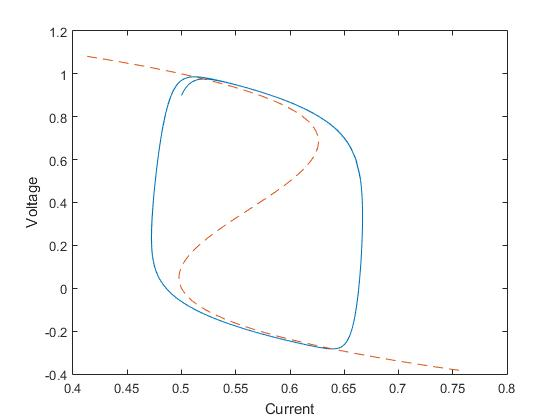
\includegraphics[width=\textwidth]{fitz_nagumo_hysteresis}
        \caption{Phase Portrait of the FitzHugh-Nagumo model. The dashed curve is the cubic nullcline.}
        \label{fitz_nagumo_hysteresis}
    \end{subfigure}
    ~ %add desired spacing between images, e. g. ~, \quad, \qquad, \hfill etc. 
    %(or a blank line to force the subfigure onto a new line)
    \begin{subfigure}[t]{0.49\textwidth}
        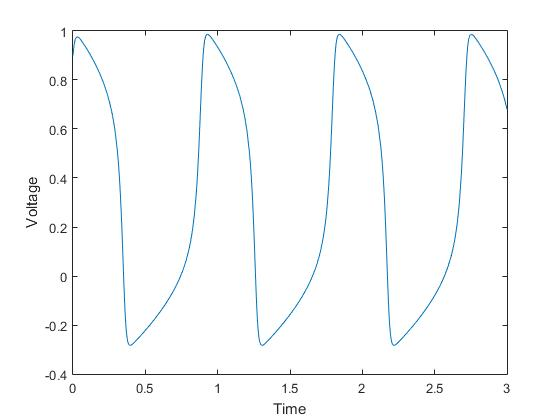
\includegraphics[width=\textwidth]{fitz_nagumo}
        \caption{Voltage oscillations against time.}
        \label{f_n}
    \end{subfigure}
\caption{FitzHugh-Nagumo model with unstable unique rest point.}
\label{fitz-nagumo}
\end{figure}

The limit cycle behaviour of the current and voltage in the phase plane reveals a hysteresis characteristic very similar to a relay element. Approximating the relationship between $w$ and $v$ as a relay could simplify the FitzHugh-Nagumo equations. This means the voltage would be the output signal from the relay, while the input signal is the current, as shown in Figure \ref{fn_transfer}. 

\begin{figure}
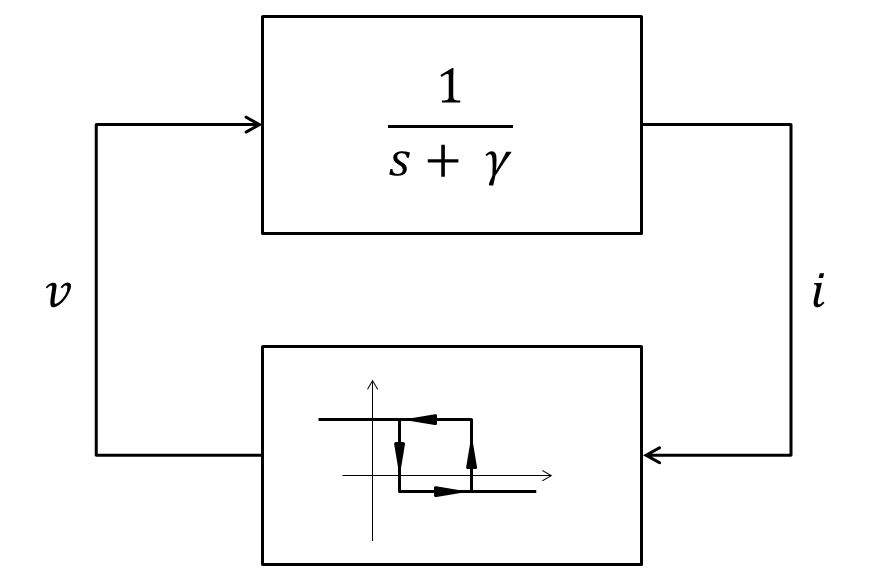
\includegraphics[width = 0.5\textwidth]{fitz_relay_transfer}
\caption{Relay feedback system approximation of FitzHugh-Nagumo.}
\label{fn_transfer}
\end{figure}

At this point, there are several parameters such as the state-space matrices ($A, B, C$), the relay element ($d_1, d_2, \epsilon_1, \epsilon_2$) and voltage behaviour ($T, \tau$) , that can be modified in order to replicate the behaviour of the FitzHugh-Nagumo model. A few ways of exploring these are:
\begin{enumerate}
\item Fixing the state-space equations according to the FitzHugh-Nagumo equations and match the voltage oscillations over time. The dependent variable are $\epsilon_1$ and $\epsilon_2$.
\item Fixing the state-space equations according to the FitzHugh-Nagumo equations and match the hysteresis. The dependent variables are $T$ and $\tau$.
\item Match the hysteresis and the voltage oscillations, allowing the state-space equations to adjusted. 
\end{enumerate}

The above methods are explored further in the next few sections. 

\subsection{Dependent variables: $\epsilon_1 $ and $\epsilon_2$}

Converting the FitzHugh-Nagumo equations to state space form, with $x$ as the current,  $u$ as the voltage output and setting the relay input-output relationship as $y = e$:
\begin{align}
\dot{x} &= \tfrac{1}{2}x + u \\
y &= x
\end{align}
The state-space matrices are $A = -\tfrac{1}{2}, B = C = 1$. Matching the voltage magnitude in Figure \ref{fitz-nagumo}, $d_1 = 0.9864, d_2 = 0.2829$. Matching the time period, $T = 0.9104, \tau = 0.4496$ (approximations). Now the dependent variables can be found by evaluating equation \ref{theorem5_1}, yielding $\epsilon_1 = 0.5442$ and $\epsilon_2 = 0.8318$. Furthermore, the initial condition $a1$ and the stability of the limit cycle can also be evaluated. The asymmetric limit cycle turns out to be stable, and the resulting behaviour is shown in Figure \ref{fn_match_voltage_time}. Clearly, the phase portrait is not very similar to the the FitzHugh-Nagumo model.


\begin{figure}[h!]
    \centering
    \begin{subfigure}[t]{0.49\textwidth}
        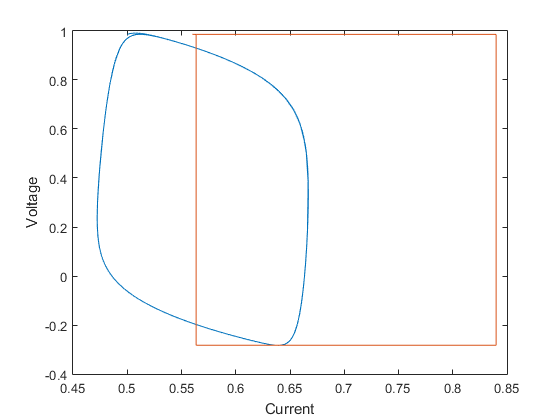
\includegraphics[width=\textwidth]{fitz_relay_match_time_period_phase_potrait}
        \caption{Phase Portrait of relay matching voltage-time.}
        \label{fn_match_voltage_time_pp}
    \end{subfigure}
    ~ %add desired spacing between images, e. g. ~, \quad, \qquad, \hfill etc. 
    %(or a blank line to force the subfigure onto a new line)
    \begin{subfigure}[t]{0.49\textwidth}
        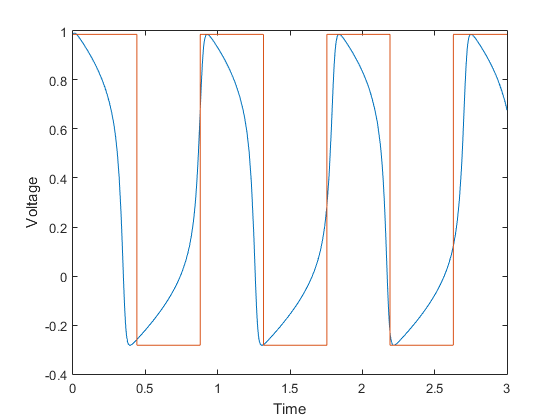
\includegraphics[width=\textwidth]{fitz_relay_match_time_period_voltage_time}
        \caption{Voltage oscillations against time.}
        \label{fn_match_voltage_time_vt}
    \end{subfigure}
\caption{Relay approximation of FitzHugh-Nagumo by matching voltage characteristics (orange). FitzHugh-Nagumo (blue).}
\label{fn_match_voltage_time}
\end{figure}



\subsection{Dependent variables: $ T $ and $ \tau $}

Using the same state-space matrices defined in the previous section, and by matching the phase portrait of Figure \ref{fitz-nagumo} sets the variables $d_1 = 0.9826, d_2 = 0.2829, \epsilon_1 = 0.4766, \epsilon_2 = 0.6666$. Here the maximum and minimum values of the hysteresis have been used. The resulting system's time variables are a bit more involved to evaluate. Modelling the system in Simulink, results Figure \ref{fn_match_hysteresis}. It is clear that the time period of the voltage oscillations are not matched. 

\begin{figure}[h!]
    \centering
    \begin{subfigure}[t]{0.49\textwidth}
        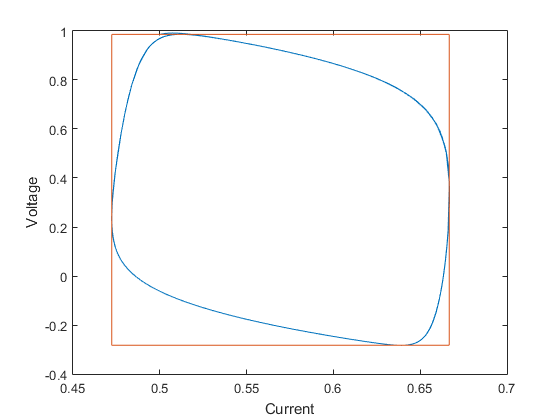
\includegraphics[width=\textwidth]{fitz_relay_match_hysteresis_phase_potrait}
        \caption{Phase Portrait of relay matching hysteresis.}
        \label{fn_match_hysteresis_pp}
    \end{subfigure}
    ~ %add desired spacing between images, e. g. ~, \quad, \qquad, \hfill etc. 
    %(or a blank line to force the subfigure onto a new line)
    \begin{subfigure}[t]{0.49\textwidth}
        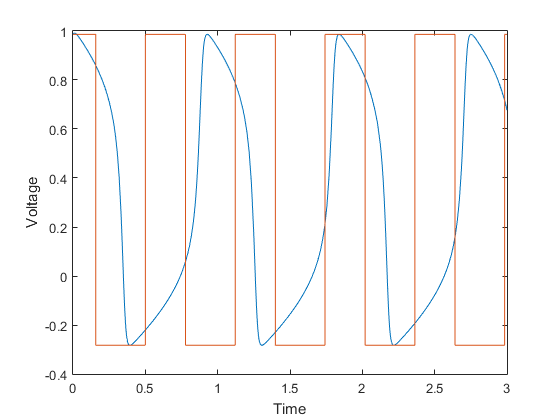
\includegraphics[width=\textwidth]{fitz_relay_match_hysteresis_voltage_time}
        \caption{Voltage oscillations against time.}
        \label{fn_match_hysteresis_vt}
    \end{subfigure}
\caption{Relay approximation of FitzHugh-Nagumo by matching hysteresis characteristics (orange). FitzHugh-Nagumo (blue).}
\label{fn_match_hysteresis}
\end{figure}

\subsection{Dependent variable : $A$}
By matching the voltage-time characteristics and the hysteresis characteristics, and by fixing the variables $B$ and $C$, the variable that needs to adjust is $A$. Rearranging for $A$ in equation \ref{theorem5_1} is not possible, and so numerical methods must be used to find $A$. One method is to rearrange all the terms into the left hand side and then find the zero crossing when $A$ is varied. Using this approach, the relay feedback system's behaviour is shown in Figure \ref{f_n_change_A}. Surprisingly, this system did not have the same time period, which suggests that perhaps there were some numerical mistakes, which needs further investigation.

\begin{figure}[h!]
    \centering
    \begin{subfigure}[t]{0.49\textwidth}
        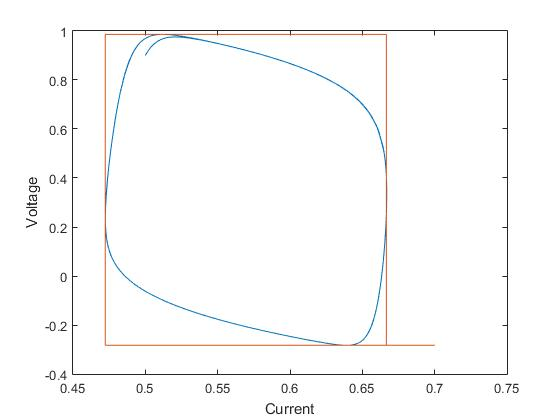
\includegraphics[width=\textwidth]{fitz_relay_change_A_hysteresis}
        \caption{Phase Portrait of relay with dependent variable A.}
        \label{fn_match_voltage_time_pp}
    \end{subfigure}
    ~ %add desired spacing between images, e. g. ~, \quad, \qquad, \hfill etc. 
    %(or a blank line to force the subfigure onto a new line)
    \begin{subfigure}[t]{0.49\textwidth}
        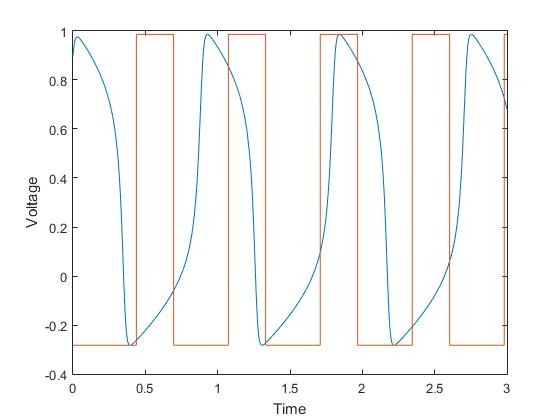
\includegraphics[width=\textwidth]{fitz_relay_change_A_voltage_time}
        \caption{Voltage oscillations against time.}
        \label{fn_match_voltage_time_vt}
    \end{subfigure}
\caption{Relay approximation of FitzHugh-Nagumo by varying A (orange). FitzHugh-Nagumo (blue).}
\label{fn_match_voltage_time}
\end{figure}


In summary, it has been shown that relay feedback systems can be used to further simplify the Hodgkin-Huxley model. There were two other variables ($B$ and $C$) that were not investigated. However, it could expected that with more degrees of freedom, the relay feedback system can be tuned to match the phase portrait and voltage-time characteristics better.


\section{Goodwin oscillator and relay feedback}
The Goodwin oscillator is a biochemical oscillator based on negative feedback alone \cite{fall}. It describes the mechanism of how mRNA, protein and end product interact. Written in their non-dimensional form \cite{fall}, the Goodwin oscillator's kinetic equations are:
\begin{align}
\frac{dx_1}{dt'} &= \frac{1}{1 + x_3^p} - b_1x_1 \\
\frac{dx_2}{dt'} &= b_2(x_1 - x_2) \\
\frac{dx_3}{dt'} &= b_3(x_2 - x_3) \\
\end{align}

It is interesting to note that there is only one non-linear term in these equations. Furthermore, this nonlinear term $(\frac{1}{1 + x_3^p})$, becomes a relay with no hysteresis as $p \rightarrow \infty$. Writing the above equations into state-space form with relay feedback yields Figure \ref{goodwin_transfer} and the equations below.

\begin{figure}
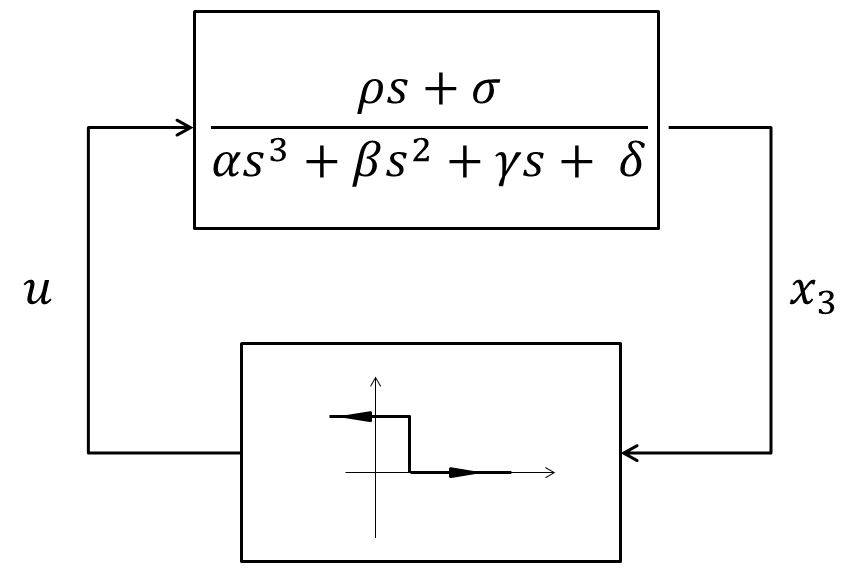
\includegraphics[width = 0.5\textwidth]{goodwin_relay_transfer}
\caption{Relay feedback system approximation of Goodwin oscillator. }
\label{goodwin_transfer}
\end{figure}

The state-space equations are :
\begin{align}
\begin{bmatrix}
	\dot{x}_1 \\ \dot{x}_2 \\ \dot{x}_3
	\end{bmatrix}
	&= \begin{bmatrix}
	-b_1 & 0 & 0 \\
	b_2 & -b_2 & 0 \\
	0 & b_3 & -b_3 \\
	\end{bmatrix}
	\begin{bmatrix}
	x_1 \\ x_2 \\ x_3 \\
	\end{bmatrix}
	+ 
	\begin{bmatrix}
	1 \\ 0 \\ 0
	\end{bmatrix}
	u \\
	y &= \begin{bmatrix}
	0 & 0 & 1 \\
	\end{bmatrix}
	\begin{bmatrix}
	x_1 \\x_2 \\x_3\\
	\end{bmatrix}
\end{align} 

The transfer function from $x_1$ to $y$,is 
 $$G(s) = C(sI-A)^{-1}B = \frac{b_2b_3 -b_3 -s}{s^3 + (b_1 + b_2 + b_3)s^2 + (b_1b_2 + b_2b_3 + b_1b_3) + b_1b_2b_3}$$

Assuming $b_1 = b_2 = b_3 = b$ simplifies calculations.  \cite{fall} explains how for $p>8$, $b$ can be chosen to be small enough to cause oscillations in the system. The relay element has no hysteresis ($\epsilon = 0$) and the relay outputs are $d_2 = 1$ and $d_1 = 0$. Hence with the three remaining parameters $b,T$ and $\tau$ we need to satisfy equation \ref{theorem5_1}:

\begin{equation}
\label{goodwin_theorem5_1}
\begin{cases}
	        C(I - \Phi)^{-1}( - \Gamma_2) = 0\\
	        C(I - \Phi)^{-1}(-\Phi_1\Gamma_2) = 0\\
	              
	            \end{cases}
\end{equation}

\begin{equation}
\Phi = e^{As} = \mathcal{L}^{-1}\left((sI-A)^{-1}\right) = e^{-bt} 
\begin{bmatrix}
1 & 0 & 0 \\ bt & 1 & 0 & \\ b^2t^2 & bt & 1 \\ 
\end{bmatrix}\\
\end{equation}
\begin{equation}
(I-\Phi)^{-1} = \frac{1}{1-e^{-bt}}
\begin{bmatrix}
1 & 0 & 0 \\
\frac{bte^{-bt}}{1-e^{-bt}} & 1 & 0 \\
\frac{b^2t^2e^{-bt}}{(1 - e^{-bt})^2} &\frac{bte^{-bt}}{1-e^{-bt}} & 1 \\
\end{bmatrix} 
\end{equation}

\begin{equation}
C(I-\Phi)^{-1} = \frac{1}{1-e^{-bt}}
\begin{bmatrix}\frac{b^2t^2e^{-bt}}{(1 - e^{-bt})^2} &\frac{bte^{-bt}}{1-e^{-bt}} & 1 \\
\end{bmatrix} = \frac{1}{1-e^{-bt}} \begin{bmatrix}
\beta_1 & \beta_2 & 1\\
\end{bmatrix}
\end{equation}

\begin{equation}
\Gamma_2 = \int_{0}^{T-\tau}
\begin{bmatrix}
1 \\ bte^{-bt} \\ b^2t^2e^{-bt} \\
\end{bmatrix}
= \begin{bmatrix}
T-\tau \\ -\frac{e^{-b(T-\tau)}}{b}\left(b(T-\tau) + 1 \right)\\
\frac{2}{b^2} - \frac{e^{-b(T-\tau)}}{b^2}\left(b^2(T-\tau)^2 + 2b(T-\tau) + 2\right)\\
\end{bmatrix} = \begin{bmatrix}
T-\tau \\ \alpha_1 \\ \alpha_2
\end{bmatrix}
\end{equation}
%\begin{equation}
%-\Phi_1\Gamma_2 = e^{-b\tau}\begin{bmatrix}
%T-\tau\\
%(\tau - T)b\tau + \tfrac{1}{b^2}e^{-b(T-\tau)}\left(b(T-\tau) + 1\right) \\
%(\tau - T)b^2\tau^2 + \tau e^{-b(T-\tau)}\left(b(T-\tau) + 1\right) + \tfrac{1}{b^2}e^{-b(T-\tau)}\left(b^2(T-\tau)^2 + 2b(T-\tau) + 2\right) - \frac{2}{b^2}
%\end{bmatrix}
%\end{equation}

\begin{equation}
\Phi_1\Gamma_2 =  e^{-b\tau}\begin{bmatrix}
T-\tau\\ b\tau(T-\tau) + \alpha_1 \\
b^2\tau^2(T-\tau) + b\tau\alpha_1 + \alpha_2\\
\end{bmatrix}
\end{equation}


\begin{equation}\label{hurrah}
C(I-\Phi)^{-1}\Gamma_2 = \frac{1}{1-e^{-bt}}\left(\beta_1 (T-\tau) + \beta_2\alpha_1 + \alpha_2\right) = 0
\end{equation}

\begin{equation} \label{hurra}
C(I-\Phi)^{-1}\Phi_1\Gamma_2 = \frac{e^{-b\tau}}{1-e^{-bt}}\left(\beta_1(T-\tau) + \beta_2(b\tau(T-\tau) + \alpha_1) + b^2\tau^2(T-\tau) + b\tau\alpha_1 + \alpha_2\right) = 0
\end{equation}


Here we have two equations (\ref{hurrah} and \ref{hurra}) and three variables. This reveals that there are many solutions depending on choosing a specific value for one of the variables. It still be difficult to solve the equations. Further work into exploring these equations will give more insight regarding this.

\section{Conclusions}
\begin{itemize}
\item Relay feedback approximation for FitzHugh-Nagumo model was investigated and found to be able to replicate most of the behavior. Some calculations need to be checked again. 
\item Relay feedback approximation for Goodwin Oscillator was investigated, however, the equations became quite involved. Further work is required here to gain better insight on how the approximation will match the real model. 
\end{itemize}


\begin{thebibliography}{9}

\bibitem{astrom1995}
K.J.\r{A}str\"{o}m , (1995) \emph{Oscillations in systems with relay feedback}. IMA Vol. Math. Appl. : Adap. Control, Filtering, Signal Processing, Volume 74, Pages 1-25. 

\bibitem{keener}
J.Keener and J.Sneyd, \emph{Mathematical Physiology}. Springer-Verlag New York. Volume 8/I. Second Edition. ISBN 978-0-387-75846-6. 

\bibitem{fall}
C.P.Fall, E.S.Marland, J.M.Wagner, J.J.Tyson, \emph{Computational Cell Biology}. Springer. Volume 20. ISBN 0-387-95369-8. 

\end{thebibliography}

\end{document}